\documentclass[11pt,nonblindrev,fleqn]{article}
\pagestyle{plain}

%\include{epsf}
\include{amsfonts}
\usepackage{graphicx}
\usepackage{amssymb,amsmath}
\usepackage{mathrsfs,threeparttable,lscape,subfigure,float,booktabs,enumerate,multirow,epstopdf,longtable}
\usepackage{algorithmic,xcolor}
\usepackage[linesnumbered,boxed,ruled]{algorithm2e}

%hyperlink colour setting
\usepackage[colorlinks,linkcolor=blue,anchorcolor=blue,citecolor=blue]{hyperref}
\def\sectionautorefname{Section}%
\def\figureautorefname{Fig.}%
\def\tableautorefname{Table}%
\def\algorithmautorefname{Algorithm}%


% table-related package
\usepackage{bigstrut,bigdelim,multirow}
\usepackage{booktabs}

%\usetikzlibrary{shapes,snakes}
%\newcommand{\USA}{\USAmap}

% Natbib setup for author-year style
\usepackage{natbib}
 \bibpunct[, ]{(}{)}{,}{a}{}{,}%
 \def\bibfont{\small}%
 \def\bibsep{\smallskipamount}%
 \def\bibhang{24pt}%
 \def\newblock{\ }%
 \def\BIBand{and}%

% Set page dimensions
\evensidemargin -.5in
\oddsidemargin -.5in
\textwidth 7.5in
\topmargin -0.5in
\textheight 9in

\newcommand{\singlespace}{\renewcommand{\baselinestretch}{1}\small\normalsize}
\newcommand{\doublespace}{\renewcommand{\baselinestretch}{1.5}\small\normalsize}


\begin{document}


\singlespace

\begin{titlepage}
\title{A hybrid algorithm for large-scale service network design considering heterogeneous fleet}
\author{Zujian Wang$^{1,2}$, Mingyao Qi$^{2}$, Chun Cheng$^3$%
\\ \footnotesize{$^{1}$Department of Industrial Engineering, Tsinghua University, Beijing 100084, China}%
\\ \footnotesize{$^{2}$Research Center on Modern Logistics, Graduate School at Shenzhen,}
\\ \footnotesize{Tsinghua University, Shenzhen 518055, China}%
\\ \footnotesize{$^{3}$Department of Mathematics and Industrial Engineering and CIRRELT,}
\\ \footnotesize{Polytechnique Montr{\'e}al and CIRRELT, Montr{\'e}al H3C 3A7, Canada}%
}

\date{} % version 11
\end{titlepage}
\maketitle

%\newpage

\abstract{
Service network design addresses decisions related to transportation services selection and origin-to-destination commodity flow distribution. In this paper, we consider the usage of heterogeneous fleet to provide services for huge transportation network. We propose both arc-based and cycle-path models to formulate the problem. A hybrid algorithm is presented to solve large-scale instances. The method includes pricing and cutting techniques to achieve stronger lower bounds, as well as a local search algorithm to obtain high-quality solutions. Computational study indicates the effectiveness and efficiency of the proposed algorithm when compared with the state-of-the-art solver CPLEX.
}

\vspace{.25in}

\noindent {\bf Keywords:} service network design; heterogeneous fleet; column generation; cutting plane; local search

%\newpage

%%%%%%%%%%%%%%%%
% INTRODUCTION %
%%%%%%%%%%%%%%%%

\doublespace
%\singlespace
\section{Introduction}
Freight transportation plays an increasingly important role because of rapid development of e-commerce. Carriers are facing tremendous pressure from growing competition and start to pay more attention to optimize their transportation network. Service network design (SND) formulations address issues related to the tactical planning for consolidation-based freight transportation systems. Specifically, such formulations make decisions on selecting transportation services and distributing origin-destination (O-D) commodity flow. Network links represent services with operational assets (e.g. vehicles, crews and power units) in SND formulations. Asset management concentrates on the operation and schedule of assets which require balance at each terminal in order to be available for services.

%1. heterogeneous fleet; 2. large-scale;
Most researchers assume that transportation system is serviced by homogenous assets which have the same property. Nevertheless, it is a common practice to employ heterogeneous fleet in transportation and logistics management for carriers. In the literature, only a small amount of efforts are devoted to considering heterogeneous fleet, e.g. \cite{Kim1999Multimodal} and \cite{li2017design}. Moveover, with the improvement of logistics infrastructure, carriers are confronted with increasingly huge transportation network. Since service network design problem is NP-hard, it is difficult to find a feasible solution for large-scale instances. Therefore, there is an urgent need for efficient algorithms to reduce costs for carriers in real-life application.

Our goal of this paper is to address this issue related to heterogeneous assets and take vehicles as an example to formulate service network design problem. Furthermore, efficient algorithms are introduced to help carriers reduce logistics-related costs when dealing with huge transportation network. Specifically, this paper makes the following contributions to the literature: First, we present both arc-based and cycle-path formulations for service network design considering heterogeneous fleet. Second, a hybrid algorithm including column generation, cutting plane and local search methods is introduced to solve large-scale instances. Moreover, the proposed algorithm provides high-quality both lower bounds and feasible solutions efficiently, and outperforms CPLEX running 10 hours of CPU time.

The outline of this paper is as follows. In \autoref{review}, a brief literature review is elaborated. We describe the problem and propose both arc-based and cycle-path formulations in \autoref{formulation}. \autoref{method} is devoted to the proposed hybrid algorithm, whereas experimental results is presented in \autoref{experiment}. Concluding remarks is given in \autoref{conclusion}.

\section{Literature review}\label{review}
% 1.asset management 2.arc, cycle structure models 3.large-scale 4.heterogenerous fleets
Service network design contains the tactical planning decisions on selecting transportation services to satisfy O-D demands which is generally formulated as fixed-cost capacitated multicommodity network design problem (CMND), see \cite{Magnanti1984Network} and \cite{Minoux1989Networks}. In addition to scheduling services and distributing flow, asset management is marginally considered in \cite{Crainic2000Service}, \cite{Smilowitz2002Deferred} and \cite{crainic2003long}. Since carriers attach increasing importance to utilize assets economically and efficiently, SND with asset management attracts increasing attention in the literature \citep{Andersen2009bService,Teypaz2010A}.   Afterwards design-balanced constraints are proposed by \cite{Pedersen2009Models}, which state that the number of assets entering each terminal must equal the number of leaving. The design-balanced constraints induce a cyclic structure for the assets movements to complete service operations and flow distribution.

With respect to the way of formulating SND, it is general to propose arc-based formulations in the literature. While \cite{Andersen2009bService} present four alternative formulations and analyze strengths and weaknesses of each formulation. The experimental results show that formulations based on cycle variables outperform other formulations in both solution quality and time. However, the number of generated cycles grows exponentially and requires more efficient enumeration algorithm. Consequently, \cite{Andersen2011Branch} propose an efficient branch-and-price scheme for the cycle-based formulation to avoid the enumeration of cycles. Their algorithm contains two subproblems for the dynamical construction of paths for commodities and cycles for vehicles.

Since the SND problem is NP-hard, heuristic methods are preferred choices. \cite{Pedersen2009Models} present a two-phase tabu search meta-heuristic framework for the arc-based formulation. The proposed algorithm includes exploration phase to build neighborhoods and feasibility phase to implement an infeasibility-monitoring procedure for reaching good feasible solutions. \cite{Teypaz2010A} present a three-step decomposition heuristic to solve large-scale freight transportation formulation and build comprehensive solutions for real-life size instances. \cite{VuDucToulouse} propose a three-phase meta-heuristic method combining neighbourhood-based and exact methods. Additionally, computational results on large-scale benchmark instances indicate the efficiency of the algorithm. Another meta-heuristic combining a cutting-plane scheme to obtain lower bound and a variable fixing procedure to cut down the dimension of the problem is introduced in \cite{Chouman2015Cutting}. \cite{Crainic2016Service} propose a new service network design model with resource constraints and design a solution approach combining column generation and slope scaling methods to find high-quality solutions.

 Only a single asset type is considered in the aforementioned literature. As for heterogeneous assets, especially multiple types of vehicles, \cite{Kim1999Multimodal} introduce three different but equivalent formulations and their potentially significant difference in computational time. They also present two sets of valid inequalities to strengthen lower bounds. However, no efficient algorithm is mentioned to solve those formulations in that paper. \cite{li2017design} propose a tabu search based meta-heuristic to solve arc-based formulation for design-balanced capacitated multicommodity network design with heterogeneous assets. However, the numbers of each fleet type employed by each service are not decided explicitly in their formulation. Moreover the scale of those experimental instances solved by the proposed algorithm cannot satisfy the real-life demand. The biggest instance in that paper only considers 25 nodes, 50 commodities and 215 arcs.

\section{Problem statement and mathematical formulation}\label{formulation}
In this section, we describe the problem and propose two equivalent formulations based on arc and cycle-path respectively.

\subsection{Problem description}
Since most literature assume homogeneous fleet is employed which may not accord with the common practices, we take heterogeneous fleet into consideration in this paper. The example network with heterogeneous fleet is shown in \autoref{Fig1}. Under this assumption, the number of different type of vehicles should be decided on each arc. In \autoref{Fig1}, there are two types of fleet providing services and arcs in solid line are labeled by the number of specific type of vehicles. At each node the numbers of same type of vehicles entering and leaving equals. A cycle consists of a sequence of arcs satisfying design-balance requirements of the same type of vehicles, e.g., $\{ (A,D),(D,C),(C,B),(B,A) \}$. A path starts at the origin of a commodity and ends at its destination. Suppose there is a commodity with origin $A$ and destination $G$, thus $\{ (A,D),(D,G) \}$ and $\{ (A,D),(D,F),(F,G) \}$ are two paths. Note that arc $(A,D)$ employs both two types of vehicles to provide transportation services. Dashed-line arcs like $(E,A)$, $(C,F)$ and $(G,E)$ mean they are not selected as a service to open.

\begin{figure}[H]
\setlength{\abovecaptionskip}{-5pt}
\setlength{\belowcaptionskip}{-5pt}
\centering
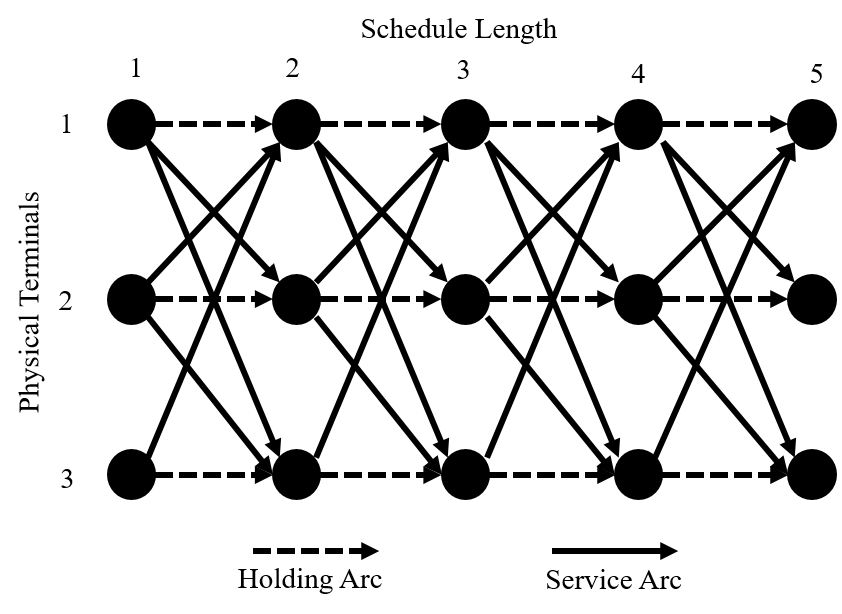
\includegraphics[width=0.4\linewidth]{F1.png}
\caption{Example of heterogeneous fleet}
\label{Fig1}
\end{figure}

Given a directed graph $G=(N,A)$ with node set $N$ and arc set $A$. Each commodity $k$ in commodity set $K$ has a known demand $d^k$ to be transited from its origin node $o(k)$ to destination node $d(k)$. Let $F$ denote the set of fleet types and each type $f\in F$ has a certain capacity $u^f$. There is no limit to the number of each types of vehicles.

\subsection{Arc-based formulation}
Let  $h_{ij}^f$ denote the fixed cost of utilizing fleet type $f\in F$ with respect to arc $(i,j)$. The unit flow cost for transporting commodity $k\in K$ on arc $(i,j)$ is denoted $c_{ij}^k$. We define $N_i^+= \{j\in N|(i,j)\in A\},N_i^-= \{j\in N|(j,i)\in A\}$. For each commodity $k$ and node $i$, define
\begin{equation*}
\omega_i^k= \left\{
\begin{aligned}
d^k&  & if \ i=o(k) \\
-d^k&  & if \ i=d(k) \\
0&  & otherwise
\end{aligned}
\right.
\end{equation*}

Two sets of decision variables are defined as follows.
\begin{itemize}
  \item Continuous variable: $x_{ij}^k$ represents the amount of flow with respect to commodity $k\in K$ on arc $(i,j)\in A$;
  \item Integer variable: $y_{ij}^f$ denotes the number of fleet type $f\in F$ that provide transportation services on arc $(i,j)\in A$.
\end{itemize}

The model is formulated as follows:
\begin{align}
  \min &  \sum_{k\in K}\sum_{(i,j)\in A} c_{ij}^k x_{ij}^k + \sum_{f\in F}\sum_{(i,j)\in A}h_{ij}^f y_{ij}^f   \label{objA}  \\
  \rm{s.t.} \nonumber  \\
         &  \sum_{j\in N_i^+}x_{ij}^k - \sum_{j\in N_i^-}x_{ji}^k = w_i^k     \quad     \forall i\in N, \forall k\in K,     \label{demandA}  \\
         &   \sum_{j\in N_i^+}y_{ij}^f - \sum_{j\in N_i^-}y_{ji}^f = 0  \quad     \forall i\in N, \forall f\in F,   \label{dbA} \\
         &   \sum_{k\in K}x_{ij}^k \leq \sum_{f\in F}u^f y_{ij}^f  \quad  \forall (i,j)\in A,   \label{capacityA} \\
         &    x_{ij}^k \geq 0  \quad  \forall (i,j)\in A, \forall k\in K,   \label{xA} \\
         &   y_{ij}^f \in Z_0^+  \quad  \forall (i,j)\in A,\forall f\in F, \label{yA}
\end{align}

The objective function (\ref{objA}) minimizes the sum of the total commodity flow costs and the fixed costs for selecting and operating transportation service with respect to heterogeneous fleet. Constraints (\ref{demandA}) represent the flow conversation relations for each node and each commodity. Equations (\ref{dbA}) are the design-balance constraints, which ensure the same number of each type of vehicles entering and leaving a node. Through Constraints (\ref{capacityA}), we enforce the total flow cannot exceed the total capacity provided by all vehicles on each arc. Finally, variable-type restrictions appear in Constraints (\ref{xA}) and (\ref{yA}).

\subsection{Cycle-path formulation}
Let $Q^f$ represent the set of all design cycle with respect to fleet type $f\in F$. And we define the set of all paths with respect to commodity $k\in K$ as $P^k$. Two sets of decision variables are given as follows.
\begin{itemize}
  \item Cycle integer variables: $y_q^f$ denotes the number of vehicle type $f$ used by cycle $q\in Q^f$;
  \item Path continuous variables: $x_p^k$ denotes the volume of commodity $k$ on path $p\in P^k$.
\end{itemize}
We define two sets of indicator variables:
\begin{itemize}
  \item $\alpha_{ij}^q$: equals 1 if arc $(i,j)$ is included in cycle $q$, and 0 otherwise;
  \item $\delta_{ij}^p$: equals 1 if arc $(i,j)$ is included in path $p$, and 0 otherwise.
\end{itemize}

The fixed cost of cycle $q$ with respect to fleet type $f$ is denoted $h_q^f$, which equals $\sum_{(i,j)\in A} h_{ij}^f \alpha_{ij}^q$. Similarly, the flow cost of path $p$ with respect to commodity $k$ is denoted $c_p^k$, which equals $\sum_{(i,j)\in A} c_{ij}^k \delta_{ij}^p$.
\begin{align}
  \min &    \sum_{k\in K}\sum_{p\in P^k}c_p^k x_p^k +  \sum_{f\in F}\sum_{q\in Q^f}h_q^f y_q^f  \label{objCP}    \\
         & \rm{s.t.} \nonumber \\
         &     \sum_{k\in K}\sum_{p\in P^k}\delta_{ij}^p x_p^k \leq  \sum_{f\in F}\sum_{q\in Q^f}u^f \alpha_{ij}^q y_q^f      \quad \forall (i,j)\in A \label{capacityCP}\\
         &     \sum_{p\in P^k}x_p^k = d^k      \quad       \forall k\in K  \label{demandCP}    \\
         &      x_p^k \geq 0        \quad       \forall p\in P^k,\forall k\in K     \label{xCP} \\
         &      y_q^f \in Z_0^+     \quad       \forall q\in Q^f, \forall f\in F    \label{yCP}
\end{align}

The objective function (\ref{objCP}) minimizes the total cost calculated as the sum of the flow costs on paths plus the fixed costs for selected cycles with respect to specific type of vehicle.Through Constraints (\ref{capacityCP}), we enforce service capacity restrictions on each arc. Constraints (\ref{demandCP}) ensure demand satisfaction corresponding to the flow conservation equations for each commodity. Finally, Constraints (\ref{xCP}) and (\ref{yCP}) give variable-type restrictions.

\subsection{Summary of two formulations}
As for comparisons of the two ways to formulate service network design problem, \cite{Andersen2009bService} have performed computational study to indicate their strengths and weaknesses. The formulation based on arc is intuitively related to the description of the problem and easier to understand. Since paths and cycles are composed of arcs, the arc-based formulation is the basis of cycle-path formulation. Furthermore, the structure of cycle-path formulation is suitable for column generation approach because each path and cycle may be added to the model as a column. In this paper, local search approach which will be introduced in \autoref{method} is based on the arc-based formulation.

\section{Solution method}\label{method}
Since service network design problem is NP-hard, it is difficult for exact algorithms to solve the large-scale instances optimally. Heuristics and metaheuristics are the preferred choices in real-life application for a minimization problem. But the drawback of heuristics algorithm is that the solutions cannot be evaluated by lower bounds. Therefore we propose a hybrid algorithm combining exact and heuristic techniques to solve the problem. The exact part mainly contains column generation and cutting plane method to obtain tight lower bounds. Moreover, we employ the linear solution provided by column-and-cut generation approach as a initial neighborhood and use local search approach to find high-quality feasible solutions. The sketch of the proposed hybrid algorithm is shown in \autoref{Methodology}.

\vspace{.15in}
\begin{algorithm}[H]
\caption{Hybrid solution method}\label{Methodology}
\LinesNumbered
\SetNlSkip{1.2em}
\While{find promising columns or cuts}
{
    column generation\;
    cutting plane\;
}
obtain lower bound\;
use the lower bound solution as initial neighborhood\;
local search approach\;
return lower bound and upper bound\;
\end{algorithm}
\subsection{Column-and-cut generation (C\&CG)}
The column generation approach has been proved to be efficient to solve cycle-path formulation by \cite{Andersen2011Branch}. With respect to cutting-plane procedure, it is also proved to be effective in calculating tight lower bounds for CMND-related problems, see \cite{Chouman2009Commodity,Chouman2016Commodity,Chouman2015Cutting}. We combine the two methods to strengthen lower bounds for the proposed formulations.

\subsubsection{Column generation (CG)}
The linear relaxation of cycle-path formulation constitutes the master problem(MP) which is solved by CG approach. Since the number of variables in the MP is exponentially increasing, it is necessary to concentrate on a restricted master problem(RMP) which contains only a subset of variables(columns) in the MP.  The CG approach starts with some necessary cycles and paths to prevent the constraints violation. We generate one path for each commodity to satisfy its O-D demand. A reversed path from the destination of each commodity to its origin is combined with the former path to constitute a cycle. Therefore, we add a path and a cycle for each commodity as the initial columns to ensure the RMP feasible. The method adds new paths and cycles dynamically to the RMP until no additional column with negative reduced cost can be found.

The dual variable values in the solution of the RMP are passed to the subproblem for generating new columns. Dual variables $\eta_{ij}$ and $\sigma_k$ are associated with constraints (\ref{capacityCP}) and (\ref{demandCP}) respectively. The reduced costs associated with cycle-related variable $y_q^f$ and path-related variable $x_p^k$ are given by:
\begin{align}
& RC_{fq} = h_q^f + \sum_{(i,j)\in A} u^f \alpha_{ij}^q \eta_{ij} = \sum_{(i,j)\in q} (h_{ij}^f + u^f \eta_{ij}) \\
& RP_{kp} = c_p^k - \sum_{(i,j)\in A} \delta_{ij}^p \eta_{ij} - \sigma_k = \sum_{(i,j)\in p} (c_{ij}^k - \eta_{ij}) - \sigma_k
\end{align}

We search for cycles and paths with negative reduced cost and add them to the RMP. The column generation procedure is presented in \autoref{CG}. When searching for the shortest cycle, we add a virtual node which is as same as the starting node as the destination node. Such that we can use the shortest path algorithm to find the shortest cycle. Note that dual variable $\eta_{ij} \leq 0$, then the arc costs may be negative when searching for the shortest cycle. Therefore, we employ the label-correcting algorithm implemented by \cite{Ahuja1993Network} to identify the shortest path.

\vspace{.25in}
\begin{algorithm}[H]
%\SetAlgoNoLine
\caption{Column generation procedure}\label{CG}
\LinesNumbered
\SetNlSkip{1.2em}
add initial sets of cycles and paths to the RMP\;
\While{find columns with negative reduced cost}
{
    solve the RMP\;
    determine dual variables $\eta_{ij}$ and $\sigma_k$\;
    \ForEach{node}
    {
        find the shortest cycle with respect to arc costs $h_{ij}^f + u^f \eta_{ij}$\;
        let $\theta_q$ denote the cost of the shortest cycle\;
        \If{$\theta_q < 0$}
        {
            add the corresponding cycle to the RMP\;
        }
    }
     \ForEach{commodity}
    {
        find the shortest path with respect to arc costs $c_{ij}^k - \eta_{ij}$\;
        let $\theta_p$ denote the cost of the shortest path\;
        \If{$\theta_p - \sigma_k < 0$}
        {
            add the corresponding path to the RMP\;
        }
    }
}
%\KwOut{best feasible solution}
\end{algorithm}

\subsubsection{Cutting plane}
The cutting plane procedure employs the generation of valid inequalities to strengthen lower bounds in relatively short time comparing with state-of-the-art software. We introduce two sets of valid inequalities including strong inequalities and cutset inequalities. Strong inequalities(SI) have been widely used to improve the quality of the LP lower bound, see \cite{Gendron1994RELAXATIONS,Gendron1999Multicommodity} and \cite{Chouman2015Cutting}. We extend SI to be suitable for the proposed formulations in our paper which are defined in inequalities (\ref{SI}). The main effects of SI is to restrict the flow of every commodity on an arc with no fleet to be 0.
\begin{align}\label{SI}
  x_{ij}^k \leq d^k \sum_{f\in F} y_{ij}^f      \quad       \forall (i,j)\in A, \forall k\in K.
\end{align}

Cutset inequalities(CI) have been used by \cite{Chouman2015Cutting} to strengthen the lower bound for CMND with design-balanced constraints. As for the circumstance of considering heterogeneous fleet, CI have been presented by \cite{Kim1999Multimodal} which are defined as
\begin{align}
    \sum_{f\in F}u^f Y_{S,\bar{S}}^f \geq  D_{S,\bar{S}}
\end{align}

where we define cutset $(S,\bar{S})$ by partitioning the node set $N$ into any nonempty subset $S$ and its complement $\bar{S}=N\backslash S$. An arc $(i,j)$ that connects node $i$ in $S$ to node $j$ in $\bar{S}$  belongs to the cutset $(S,\bar{S})$. Let $Y_{S,\bar{S}}^f$ denote the total number of type $f$ vehicles used on the cutset $(S,\bar{S})$ arcs, i.e., $\sum_{(i,j)\in (S,\bar{S})} y_{ij}^f$ for the arc-based formulation and $\sum_{q\in Q^f}\sum_{(i,j)\in (S,\bar{S})} \alpha_{ij}^q y_q^f $ for the cycle-path formulation. Let $D_{S,\bar{S}}$ denote the aggregate demand of all commodities with their origin in $S$ and destination in $\bar{S}$. CI ensure the total demand that must flow from $S$ to $\bar{S}$ will be satisfied by enough capacity on the arcs of $(S,\bar{S})$. In general, the LP solution will not violate CI. Therefore, we lift CI by using a integer rounding procedure to produce $Chv\acute{a}tal$-$Gomory$ (C-G) cuts which are proved to be valid by \cite{Kim1999Multimodal}. The impact of adding cuts on the pricing problem is negligible, thus there is no need to modify arc costs.
\begin{align}
  \sum_{f\in F} \left( \left \lceil \frac{u_f}{u_l} \right \rceil Y_{S,\bar{S}}^f  \right)  \geq \left\lceil \frac{D_{S,\bar{S}}}{u_l} \right\rceil  \quad   \forall l\in F
\end{align}
The challenge in using cutset inequalities is how to deal with large amounts of potential cutsets, it is impractical to enumerate all the associated inequalities. Moveover, it becomes more computationally expensive to lift the inequalities as the scale of the problem increases. Therefore, we only generate single-node cutset inequalities, see \cite{Chouman2016Commodity} for the details.

The dynamic generation of valid inequalities is embedded in the column generation approach. Once there exist violated cuts, column generation procedure is executed again. The price-and-cut loop stops only if neither negative reduced cost columns nor violated cuts are found.

\subsection{Local search}\label{localSearch}
Since the application of SND employing heterogeneous fleet by logistics enterprises will deal with large-scale network, it is necessary to present effective algorithms to find high-quality solutions efficiently. Therefore, we propose a two-stage local search algorithm to find feasible solutions. Based on the linear solution obtained from C\&CG approach, we consider it as a initial neighborhood to search for better solutions.

After we obtain the lower bound, C\&CG approach will provide the value of $\bar{x}_{ij}^k$ and $\bar{y}_{ij}^f$ which are defined in arc-based formulation. Then define the arc subset including arcs with nonzero flows as $A_1$, i.e., $A_1 = \{ (i,j)\in A : \sum_{k\in K} \bar{x}_{ij}^k >0 \} $, and another arc subset including arcs with nonzero vehicles as $A_2$, i.e., $A_2 =\{  (i,j)\in A : \sum_{f\in F} \bar{y}_{ij}^f >0 \}$. It is easy to find that $A_1\subseteq A_2 \subseteq A$ because of the capacity constraints. The first stage satisfies O-D demands and determines flows on each arc $(i,j)\in A_1$. The second stage ensures the balance of vehicles and provides enough capacity for flows on each arc $(i,j)\in A_2$. The corresponding formulations in two stages are defined as follows.

\subsubsection{Stage 1: flow distribution problem}
Without taking service selection and fleet assignment into account, the formulation of flow distribution problem is actually a capacitated multi-commodity minimum cost flow problem (CMCF). The values of $\sum_{(i,j)\in A_1}u^f \bar{y}_{ij}^f $ decides the capacity $u_{ij}$ of arc $(i,j)$ in $A_1$.
\begin{align}
   \min& \sum_{(i,j)\in A_1}\sum_{k\in K} c_{ij}^k x_{ij}^k     \\
   \rm{s.t.} & \nonumber \\
         &  \sum_{j\in N_i^+}x_{ij}^k - \sum_{j\in N_i^-}x_{ji}^k = w_i^k     \quad      \forall i\in N, \forall k\in K,  \\
         &  \sum_{k\in K} x_{ij}^k \leq u_{ij}      \quad    \forall (i,j)\in A_1,  \\
        &  x_{ij}^k \geq 0   \quad    \forall (i,j)\in A_1, \forall k\in K.
\end{align}

After solving the CMCF and redistributing the flow on each arc, the arcs without flow are removed from $A_1$, i.e., $A_1 = A_1 \backslash  \{ (i,j)\in A_1 : \sum_{k\in K} x_{ij}^k =0 \}$.

\subsubsection{Stage 2: fleet assignment problem}
Once completing the flow distribution and satisfying the demands of all O-D commodities, we need to assign heterogeneous fleet to provide transportation services. Let $\Omega_{ij}$ be the total flows of all commodities distributed on arc $(i,j) \in A_2$, which equals $\sum_{k\in K}x_{ij}^k$ provided by solving CMCF in the first stage. The mathematical formulation of Stage 2 defined on arc set $A_2$ is as follow:
\begin{align}
  \min & \sum_{f\in F}\sum_{(i,j)\in A_2} h_{ij}^f y_{ij}^f \\
    \rm{s.t.} & \nonumber \\
     & \sum_{j\in N_i^+}y_{ij}^f - \sum_{j\in N_i^-}y_{ji}^f = 0     \quad      \forall i\in N,\forall f\in F  \\
     & \sum_{f\in F} u^f y_{ij}^f \geq \Omega_{ij}      \quad       \forall (i,j)\in A_2   \label{cap} \\
     & y_{ij}^f \in Z_0^+       \quad       \forall (i,j)\in A_2, \forall f\in F
\end{align}

Constraints (\ref{cap}) ensure each service arc will provide sufficient vehicle capacity for the total flow.

\subsubsection{Cycle-based neighborhoods}
After the two formulations are solved, we obtain a feasible solution of the original problem. The quality of the feasible solution depends on the two arc subsets $A_1$ and $A_2$. To find promising $A_1$ and $A_2$, we introduce cycle-based neighborhoods to search for better feasible solutions. The cycle-based neighborhoods have been presented and proved to be efficient when solving CMND-related problems, see \cite{Ghamlouche2003Cycle, Ghamlouche2004Path,li2017design}.

The cycle-based neighborhoods aim at redirecting flow from one path to another, and exploring the space of arc subsets $A_1$ and $A_2$ through opening or closing some arcs. To illustrate, considering the partial network in \autoref{cycle}, there is a cycle formed by paths $\{ (A,B),(B,C),(C,F) \}$ and $\{ (A,E),(E,F)\}$. If we redirect the flow from the former to the latter, a new solution will be generated by opening arcs $(A,E),(E,F)$ and closing empty arcs $(A,B),(B,C),(C,F)$. The procedure of finding a cycle-based neighborhood can be summarized as follows.
\begin{itemize}
  \item Identify a cycle containing two paths connecting two points.
  \item Redirect the flow from one path to another and ensure that at least one open arc becomes empty.
  \item Open all formerly closed arcs in the cycle and close all formerly open arcs if they are empty after the flow redirection.
\end{itemize}

\begin{figure}[H]
\setlength{\abovecaptionskip}{-5pt}
\setlength{\belowcaptionskip}{-5pt}
\centering
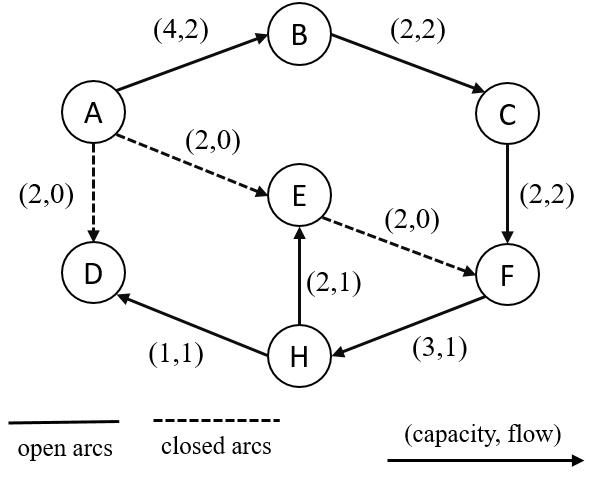
\includegraphics[width=0.5\linewidth]{F2.png}
\caption{Example of cycle in partial network}
\label{cycle}
\end{figure}

It is very important to implement an efficient procedure to find a promising neighborhood since complete evaluation of all moves is impractical, especially facing huge networks. Note that since we have to close at least one previously open arc, it seems suitable to start from a nonempty open arc $(i^*,j^*)$ with $\gamma = \sum_{k\in K} x_{i^*j^*}^k$ units of flow. Since the arc $(i^*,j^*)$ will be closed after the flow redirection, the residual capacity of any cycle associated with $(i^*,j^*)$ must be at least $\gamma$. A residual network must be built to efficiently search for low-cost cycles corresponding to promising moves without exhaustive exploration and exact evaluation.

To build such a residual network associated to $(i^*,j^*)$ and $\gamma$ units of flow redirection, we include two types of arc sets in the new network, one with positive arc cost for additional flows and the other with negative arc cost for reduced flows. Each arc in the original network will be replaced by at most two arcs $(i,j)^+$ and $(j,i)^-$ from the two arc sets respectively. Define $\bar{c}_{ij}$ as the average unit flow cost on arc $(i,j)$, i.e. $\bar{c}_{ij} = \sum_{k\in K} c_{ij}^k / |K|$. Let $\bar{F}_{ij}$ denote the average fixed cost of arc $(i,j)$ to evaluate the impact of fleet assignment because of opening or closing arcs, which equals $\sum_{f\in F}h_{ij}^f/ |F|$.

Arc $(i,j)^+$ will be included in the residual network if the residual capacity of arc $(i,j)$ is no less than $\gamma$, i.e. $ u_{ij} - \sum_{k\in K} x_{ij}^k \geq \gamma$. The cost $c_{ij}^+$ corresponding to $(i,j)^+$ approximates the additional cost of distribute $\gamma$ units of flow on arc $(i,j)$. It is calculated as the additional flow cost, plus the average fixed cost if arc $(i,j)$ is closed at present, i.e. $(i,j) \notin A_2$.
\begin{equation*}
c_{ij}^+ = \left\{
\begin{aligned}
&\bar{c}_{ij} \gamma + \bar{F}_{ij}  & & if\ (i,j) \notin A_2, \\
&\bar{c}_{ij} \gamma                 & & otherwise.
\end{aligned}
\right.
\end{equation*}

Since arc $(j,i)^-$ is employed to represent flow reduction on arc $(i,j)$, it will be included in the residual network only if the current flow on $(i,j)$ is no less than $\gamma$. Symmetrically, the cost $c_{ji}^-$ associated to $(j,i)^-$ approximates the reduced cost of decreasing $\gamma$ units of flow on arc $(i,j)$. It is calculated as the reduced flow cost, minus the average fixed cost if arc $(i,j)$ will be empty after reduction of $\gamma$ units of flow.
\begin{equation*}
c_{ji}^- = \left\{
\begin{aligned}
&-\bar{c}_{ij} \gamma - \bar{F}_{ij}  &if \ & \sum_{k\in K} x_{ij}^k = \gamma, \\
&-\bar{c}_{ij} \gamma                  &if \ &\sum_{k\in K} x_{ij}^k > \gamma.
\end{aligned}
\right.
\end{equation*}

Such a residual network aims at identifying the lowest-cost cycle containing arc $(i^*,j^*)$ to redirect $\gamma$ units of flow. Moreover, it takes into account the influence of opening or closure of arcs to search for better feasible solutions. To illustrate how to find the lowest-cost cycle in the residual network, consider the network example of \autoref{NetworkExample}. Suppose arc $(A,B)$ is the candidate arc to be closed, the residual network associated with $(A,B)$ is shown in \autoref{NetworkExample}. The average unit flow costs and fixed costs of all arcs in the example are assumed to be 2 and 3 respectively. Arcs in the residual network are labeled by their costs. Note that there are two cycles associated with arc $(A,B)$: $(A,E),(E,F),(F,C),(C,B),(B,A)$ and $(A,E),(E,B),(B,A)$. The two cycles have costs of -7 and 4, respectively. Since the former cycle has the lowest cost, 2 units of flow are moved from path $\{(A,B),(B,C),(C,F)\}$ to path $\{(A,E),(E,F)\}$. Therefore, a new neighborhood is obtained by opening arcs $(A,E),(E,F)$ and closing empty arcs $(A,B),(B,C),(C,F)$.
\begin{figure}[H]
\setlength{\abovecaptionskip}{-5pt}
\setlength{\belowcaptionskip}{-5pt}
\centering
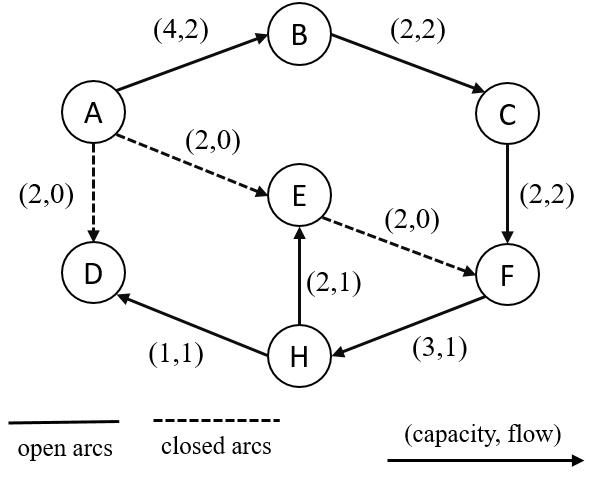
\includegraphics[width=0.9\linewidth]{F3.png}
\caption{Network example associated with $(A,B)$}
\label{NetworkExample}
\end{figure}

\subsubsection{Main local search loop}
Since each new neighborhood is associated with a candidate arc, let $A^+$ denote the candidate arcs, which equals $\{ (i,j)\in A: \sum_{k\in K} x_{ij}^k > 0 \}$. With respect to each arc $(i^*,j^*)$ in $A^+$, we build a residual network except arc $(i^*,j^*)$ and find the shortest path from $i^*$ to $j^*$ to complete the cycle. We still employ the label-correcting algorithm implemented by \cite{Ahuja1993Network} to identify the shortest path.

Note that the closure of some arcs may lead to infeasible neighboring solutions. Therefore it is necessary to check whether at least one path links the origin and destination of each commodity before comparing the cycle costs. Although it can not ensure the feasibility of the first stage when solving the flow distribution problem, it still decreases the appearance of infeasible local search moves.

Once the lowest cost cycle is found, $A_1$ is updated by the move including opening and closure of some arcs. Then we solve the flow distribution problem and update $A_1$ again by closing empty arcs. Before solving the fleet assignment problem, $A_2$ is updated by $A_1 \cup A_2$. If the two stages are both feasible, we obtain a feasible solution of the original problem. Furthermore, $A_1$ and $A_2$ in the next iteration are determined by this feasible solution. To explore more extensive search space, we assign a tabu status to the arc associated with the feasible move. The local search approach terminates if either of the two stages is infeasible or the maximum iteration is reached. The sketch of the local search algorithm is shown in \autoref{LS}.

\vspace{.25in}
\begin{algorithm}[H]
%\SetAlgoNoLine
\caption{Local search algorithm}\label{LS}
\LinesNumbered
\SetNlSkip{1.2em}
\KwIn{linear solution obtained by C\&CG}
\While{termination criterion not met}
{
    determine $A_1,A_2$ and $A^+$\;
    \ForEach{$(i^*,j^*)\in A^+$}
    {
        create residual network\;
        determine the lowest-cost cycle associated with $(i^*,j^*)$\;
    }
    find the cycle with minimum cost\;
    implement the move\;
    update $A_1$ then solve flow distribution problem, stop if infeasible\;
    update $A_1$ and $A_2$\;
    solve fleet assignment problem, stop if infeasible\;
    update the current solution\;
    assign a tabu status to $(i^*,j^*)$\;
    \If{find better solution}
    {
        update best feasible solution\;
    }
}
\KwOut{best feasible solution}
\end{algorithm}


\section{Numerical experiments and analyses}\label{experiment}
The computation study is implemented in C++, using CPLEX 12.63 as the linear programming solver. All experiments are performed using a computer with four 64-bit 2.4 GHz Intel Core processors and 4 GB of RAM, operating under Windows 10. Computing time is reported in seconds.

\subsection{Data instances}
Since there are no suitable instances available in the literature, we randomly generate 30 large-scale instances based on the classic network instance sets described in \cite{crainic2001bundle} and used in several papers (\cite{Ghamlouche2003Cycle,Pedersen2009Models} and \cite{Chouman2015Cutting}). The arc flow cost is an integer randomly generated in the interval [2,7]. The demand of each commodity is generated over [2,15]. The capacity and fixed cost of each type of fleet is a random number in the interval [2,15] and [100,300] respectively. Each instance is characterized by its numbers of fleet types, nodes, commodities and arcs, noted $|F|\in \{5,10\}$, $|N|\in \{30,35,40\}$, $|K|\in \{200,300,400\}$ and $|A|\in \{600,800\}$, respectively.

\subsection{Parameter setting}
During the process of computing lower bound, to avoid instability, we use the CPLEX recommended value, a tolerance of $10^{-6}$ for relative change in objective function value in column generation approach. That is, columns will be added only if their reduced costs is less than $-10^{-6}$.

%max iteration of local search
As for the maximum iteration of local search algorithm, we choose two instances randomly from the generated 30 instances, i.e., instance 15 and instance 23 whose properties are listed in \autoref{results} in detail. We record the change of total cost for the two instances in each local search iteration to illustrate the evolution of solution values. As \autoref{Evolution} shows, the solution values are improved very significantly in previous several iterations. But the improvement tendency of the solution value becomes weak near 50 iterations. Therefore, we set the maximum iteration number as 50.

Furthermore, we find it easy to obtain a good solution in a short time when solving the second stage in local search procedure. There is no need to solving the second stage optimally. Therefore the fleet assignment problem is solved by CPLEX with a time limit of 30 seconds.
\begin{figure}[H]
\setlength{\abovecaptionskip}{-5pt}
\setlength{\belowcaptionskip}{-5pt}
\centering
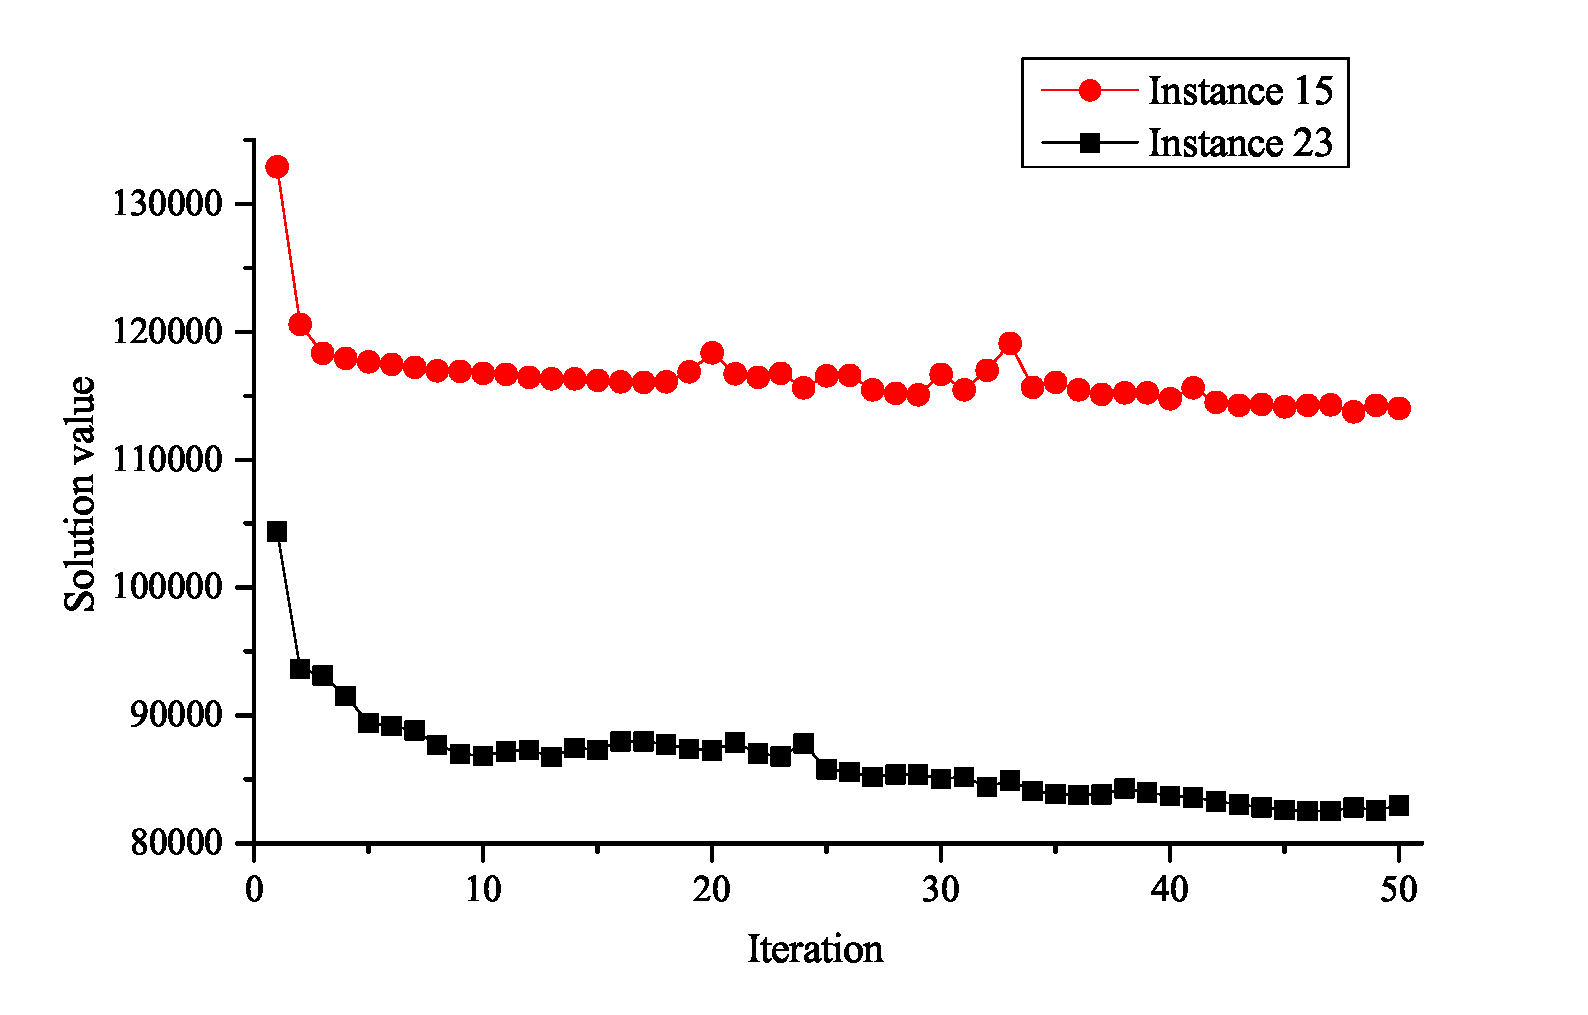
\includegraphics[width=0.8\linewidth]{F4.eps}
\caption{Evolution of solution values obtained by local search approach}
\label{Evolution}
\end{figure}

\subsection{Computational results}
The scope of the section is to evaluate the performance of the proposed solution method. In particular, We compare the results with CPLEX running 10 hours of CPU time to show clearly its effectiveness and efficiency in strengthening the lower bounds and finding high-quality feasible solutions. The comparison results with respect to 30 large-scale instances are shown in \autoref{results}. Without loss of generality, the values of all lower bound, upper bound and computing time are round to integers to show in \autoref{results}.

The lower bounds and upper bounds obtained by CPLEX running 10 hours of CPU time are shown in Column LB$_1$ and UB$_1$. Let GAP$_1$ denote the percentage gap between LB$_1$ and UB$_1$, which is calculated as $\rm \frac{UB_1 - LB_1}{UB_1}\times 100$. The lower bounds, total number of cuts and total computing time obtained by column-and-cut generation approach are displayed in column LB$_2$, Cuts and T$_1$, respectively. The percentage gap between LB$_1$ and LB$_2$ is shown in column GAP$_2$, which is calculated as $\rm \frac{LB_2 - LB_1}{LB_2}\times 100$. Column UB$_2$ and T$_2$ display the upper bounds and computing time of local search approach. Column GAP$_3$ denotes the percentage gap between UB$_1$ and UB$_2$, i.e., $\rm \frac{UB_2 - UB_1}{UB_2}\times 100$. The last column GAP$_4$ shows the percentage gap between UB$_2$ and LB$_2$, which is calculated as $\rm \frac{UB_2 - LB_2}{UB_2}\times 100$.

We calculate the distribution of four relative percentage gaps listed in \autoref{results} and show the results in \autoref{distributions}. GAP$_1$ and GAP$_4$ denote the relative gaps between lower bounds and upper bounds obtained by CPLEX and the proposed hybrid algorithm with respect to 30 instances. The gaps of most instances are more than 50 when solved by CPLEX, by contrast, the gaps of most instances are between 10 and 20 when solved by the proposed hybrid algorithm. In general, CPLEX achieves relative gap by 50.90\% on average after 10 hours of CPU time. Nevertheless, the proposed hybrid algorithm achieves relative gap by 18.14\% and only takes 2124 seconds averagely. 

\begin{table}[H]
\setlength{\abovecaptionskip}{-3pt}
\setlength{\belowcaptionskip}{5pt}
\centering
  \footnotesize
  \caption{Performance comparisons with CPLEX}
  \label{results}

% Table generated by Excel2LaTeX from sheet 'Sheet4'
\begin{tabular}{cccccccccccccccccc}
\hline
\multirow{3}[4]{*}{No.} & \multirow{3}[4]{*}{$|F|$} & \multirow{3}[4]{*}{$|N|$} & \multirow{3}[4]{*}{$|K|$} & \multirow{3}[4]{*}{$|A|$} & \multicolumn{3}{c}{CPLEX(10h)} & \multirow{3}[4]{*}{} & \multicolumn{4}{c}{Column \& cut generation } & \multirow{3}[4]{*}{} & \multicolumn{3}{c}{Local search} & \multirow{2}[3]{*}{
GAP$_4$} \bigstrut\\
\cline{6-8}\cline{10-13}\cline{15-17}      &       &       &       &       & \multirow{2}[2]{*}{UB$_1$} & \multirow{2}[2]{*}{LB$_1$} & GAP$_1$ &       & \multirow{2}[2]{*}{LB$_2$} & GAP$_2$ & \multirow{2}[2]{*}{Cuts} & \multirow{2}[2]{*}{T$_1$} &       & \multirow{2}[2]{*}{UB$_2$} & GAP$_3$ & \multirow{2}[2]{*}{T$_2$} &  \bigstrut[t]\\
      &       &       &       &       &       &       & (\%)  &       &       & (\%)  &       &       &       &       & (\%)  &       & (\%) \bigstrut[b]\\
\hline
1     & 5     & 30    & 200   & 600   & 56924 & 49789 & 12.53  &       & \textbf{50703 } & 1.80  & 243   & 167   &       & 60976 & 6.65  & 473   & 16.85  \bigstrut[t]\\
2     & 5     & 30    & 200   & 800   & 72651 & 43794 & 39.72  &       & \textbf{45007 } & 2.70  & 265   & 476   &       & \textbf{55676} & -30.49  & 534   & \textbf{19.16 } \\
3     & 5     & 30    & 300   & 600   & 128337 & 67196 & 47.64  &       & \textbf{68497 } & 1.90  & 284   & 266   &       & \textbf{79869} & -60.68  & 1275  & \textbf{14.24 } \\
4     & 5     & 30    & 300   & 800   & 111534 & 61256 & 45.08  &       & \textbf{63313 } & 3.25  & 299   & 583   &       & \textbf{75897} & -46.95  & 926   & \textbf{16.58 } \\
5     & 5     & 30    & 400   & 800   & 145367 & 80274 & 44.78  &       & \textbf{83075 } & 3.37  & 403   & 537   &       & \textbf{96035} & -51.37  & 2043  & \textbf{13.50 } \\
6     & 5     & 35    & 200   & 600   & 60604 & 52138 & 13.97  &       & \textbf{52579 } & 0.84  & 195   & 340   &       & 63426 & 4.45  & 918   & 17.10  \\
7     & 5     & 35    & 200   & 800   & 103486 & 49710 & 51.96  &       & \textbf{50371 } & 1.31  & 228   & 621   &       & \textbf{63999} & -61.70  & 579   & \textbf{21.29 } \\
8     & 5     & 35    & 300   & 600   & 166677 & 74780 & 55.13  &       & \textbf{75134 } & 0.47  & 238   & 317   &       & \textbf{85966} & -93.89  & 1705  & \textbf{12.60 } \\
9     & 5     & 35    & 300   & 800   & 150886 & 73057 & 51.58  &       & \textbf{74124 } & 1.44  & 283   & 708   &       & \textbf{88060} & -71.34  & 1268  & \textbf{15.82 } \\
10    & 5     & 35    & 400   & 800   & 169514 & 91011 & 46.31  &       & \textbf{91923 } & 0.99  & 330   & 628   &       & \textbf{106591} & -59.03  & 3180  & \textbf{13.76 } \\
11    & 5     & 40    & 200   & 600   & 136708 & 59145 & 56.74  &       & \textbf{59162 } & 0.03  & 225   & 378   &       & \textbf{69868} & -95.67  & 1608  & \textbf{15.32 } \\
12    & 5     & 40    & 200   & 800   & 140979 & 50949 & 63.86  &       & \textbf{51558 } & 1.18  & 246   & 786   &       & \textbf{64225} & -119.51  & 1166  & \textbf{19.72 } \\
13    & 5     & 40    & 300   & 600   & 205291 & 81987 & 60.06  &       & \textbf{82239 } & 0.31  & 251   & 348   &       & \textbf{94092} & -118.18  & 2207  & \textbf{12.60 } \\
14    & 5     & 40    & 300   & 800   & 152466 & 78037 & 48.82  &       & \textbf{78353 } & 0.40  & 279   & 868   &       & \textbf{92660} & -64.54  & 1968  & \textbf{15.44 } \\
15    & 5     & 40    & 400   & 800   & 210357 & 97754 & 53.53  &       & \textbf{98586 } & 0.84  & 331   & 847   &       & \textbf{113725} & -84.97  & 3360  & \textbf{13.31 } \\
16    & 10    & 30    & 200   & 600   & 54034 & 41679 & 22.86  &       & \textbf{43106 } & 3.31  & 270   & 326   &       & \textbf{53750} & -0.53  & 547   & \textbf{19.80 } \\
17    & 10    & 30    & 200   & 800   & 85816 & 39018 & 54.53  &       & \textbf{41318 } & 5.57  & 277   & 361   &       & \textbf{56274} & -52.50  & 222   & \textbf{26.58 } \\
18    & 10    & 30    & 300   & 600   & 159767 & 60743 & 61.98  &       & \textbf{63196 } & 3.88  & 368   & 236   &       & \textbf{75971} & -110.30  & 1378  & \textbf{16.82 } \\
19    & 10    & 30    & 300   & 800   & 112950 & 57601 & 49.00  &       & \textbf{61501 } & 6.34  & 342   & 835   &       & \textbf{77457} & -45.82  & 1181  & \textbf{20.60 } \\
20    & 10    & 30    & 400   & 800   & 144109 & 75363 & 47.70  &       & \textbf{80385 } & 6.25  & 447   & 696   &       & \textbf{92690} & -55.47  & 2555  & \textbf{13.28 } \\
21    & 10    & 35    & 200   & 600   & 95446 & 45739 & 52.08  &       & \textbf{46752 } & 2.17  & 338   & 279   &       & \textbf{59730} & -59.80  & 817   & \textbf{21.73 } \\
22    & 10    & 35    & 200   & 800   & 148665 & 44270 & 70.22  &       & \textbf{46056 } & 3.88  & 272   & 1062  &       & \textbf{63544} & -133.95  & 761   & \textbf{27.52 } \\
23    & 10    & 35    & 300   & 600   & 142254 & 68884 & 51.58  &       & \textbf{69931 } & 1.50  & 370   & 452   &       & \textbf{82531} & -72.36  & 1904  & \textbf{15.27 } \\
24    & 10    & 35    & 300   & 800   & 136667 & 59582 & 56.40  &       & \textbf{62267 } & 4.31  & 411   & 574   &       & \textbf{76888} & -77.75  & 1947  & \textbf{19.02 } \\
25    & 10    & 35    & 400   & 800   & 203376 & 78123 & 61.59  &       & \textbf{81104 } & 3.68  & 505   & 622   &       & \textbf{98203} & -107.10  & 2982  & \textbf{17.41 } \\
26    & 10    & 40    & 200   & 600   & 157310 & 50049 & 68.18  &       & \textbf{50306 } & 0.51  & 299   & 569   &       & \textbf{66488} & -136.60  & 1581  & \textbf{24.34 } \\
27    & 10    & 40    & 200   & 800   & 119555 & 46457 & 61.14  &       & \textbf{47406 } & 2.00  & 306   & 1048  &       & \textbf{63623} & -87.91  & 876   & \textbf{25.49 } \\
28    & 10    & 40    & 300   & 600   & 180064 & 73285 & 59.30  &       & \textbf{74031 } & 1.01  & 416   & 409   &       & \textbf{90454} & -99.07  & 2053  & \textbf{18.16 } \\
29    & 10    & 40    & 300   & 800   & 167173 & 65169 & 61.02  &       & \textbf{66717 } & 2.32  & 450   & 842   &       & \textbf{85347} & -95.87  & 2229  & \textbf{21.83 } \\
30    & 10    & 40    & 400   & 800   & 197232 & 83307 & 57.76  &       & \textbf{85543 } & 2.61  & 507   & 702   &       & \textbf{105818} & -86.39  & 2589  & \textbf{19.16 } \\
\multicolumn{5}{c}{Average}           & -     & -     & 50.90  &       & -     & \textbf{2.34 } & 323   & \textbf{563} &       & -     & \textbf{-72.29 } & \textbf{1561} & \textbf{18.14 } \bigstrut[b]\\
\hline
\end{tabular}%

\end{table}%

\subsubsection{Evaluation of column-and-cut generation approach}
\autoref{results} displays the performance of column-and-cut generation approach with respect to lower bound. Comparing with CPLEX running 10 hours, C\&CG approach finds better lower bounds in very short time. The values of GAP$_2$ being positive means C\&CG approach can find tighter lower bounds. In general, C\&CG approach achieves stronger lower bounds by 2.34\% on average comparing with CPLEX, and only takes 563 seconds averagely. 

This could signify the efficiency of C\&CG method in searching for promising columns to reduce the problem size. Then the cuts are added to strengthen the lower bound by identifying violated valid inequalities. Although the improvements are not significantly, it is still impressive considering the computing time. It only takes hundreds of seconds to outperform CPLEX running 10 hours.

\begin{table}[H]
\setlength{\abovecaptionskip}{-3pt}
\setlength{\belowcaptionskip}{5pt}
\centering
  \footnotesize
  \caption{Distribution of relative percentage gaps}
  \label{distributions}

% Table generated by Excel2LaTeX from sheet '图表'
\begin{tabular}{cccccc}
\hline
      & [10,20) & [20,30) & [30,40) & [40,50) & [50,$\infty$) \bigstrut\\
\hline
GAP$_1$ & 2     & 1     & 1     & 7     & 19 \bigstrut[t]\\
GAP$_4$ & 22    & 8     & 0     & 0     & 0 \bigstrut[b]\\
\hline
\multirow{2}[4]{*}{GAP$_2$} & [0,1.5) & [1.5,3) & [3,4.5) & [4.5,6) & [6,$\infty$) \bigstrut\\
\cline{2-6}      & 13    & 7     & 7     & 1     & 2 \bigstrut\\
\hline
\multirow{2}[4]{*}{GAP$_3$} & [$-\infty$,-120) & [-120,-80) & [-80,-40) & [-40,0) & [0,$\infty$) \bigstrut\\
\cline{2-6}      & 2     & 11    & 13    & 2     & 2 \bigstrut\\
\hline
\end{tabular}%

\end{table}%

\subsubsection{Evaluation of local search approach}
The results with respect to local search approach demonstrate its efficiency in searching for high-quality solutions for large-scale instances, which are illustrated in \autoref{results}. The improvements calculated through GAP$_3$ of several instances may exceed one hundred percentage. In general, local search approach improves the upper bounds by -72.29\% on average comparing with CPLEX, and only takes 1561 seconds averagely. The distribution of GAP$_3$ in \autoref{distributions} displays the significant improvement of upper bounds by local search approach.

\autoref{threeUB} shows the comparative upper bounds of CPLEX and local search approach. We display both the initial solution values at the first iteration and the best solution values obtained by local search approach. A majority of the initial solution values line is under the line of the best solution value by CPLEX. Therefore, it confirms that the linear solutions obtained by C\&CG approach provide good neighborhood for local search approach to find high-quality initial solutions.

\begin{figure}[H]
\setlength{\abovecaptionskip}{-5pt}
\setlength{\belowcaptionskip}{-5pt}
\centering
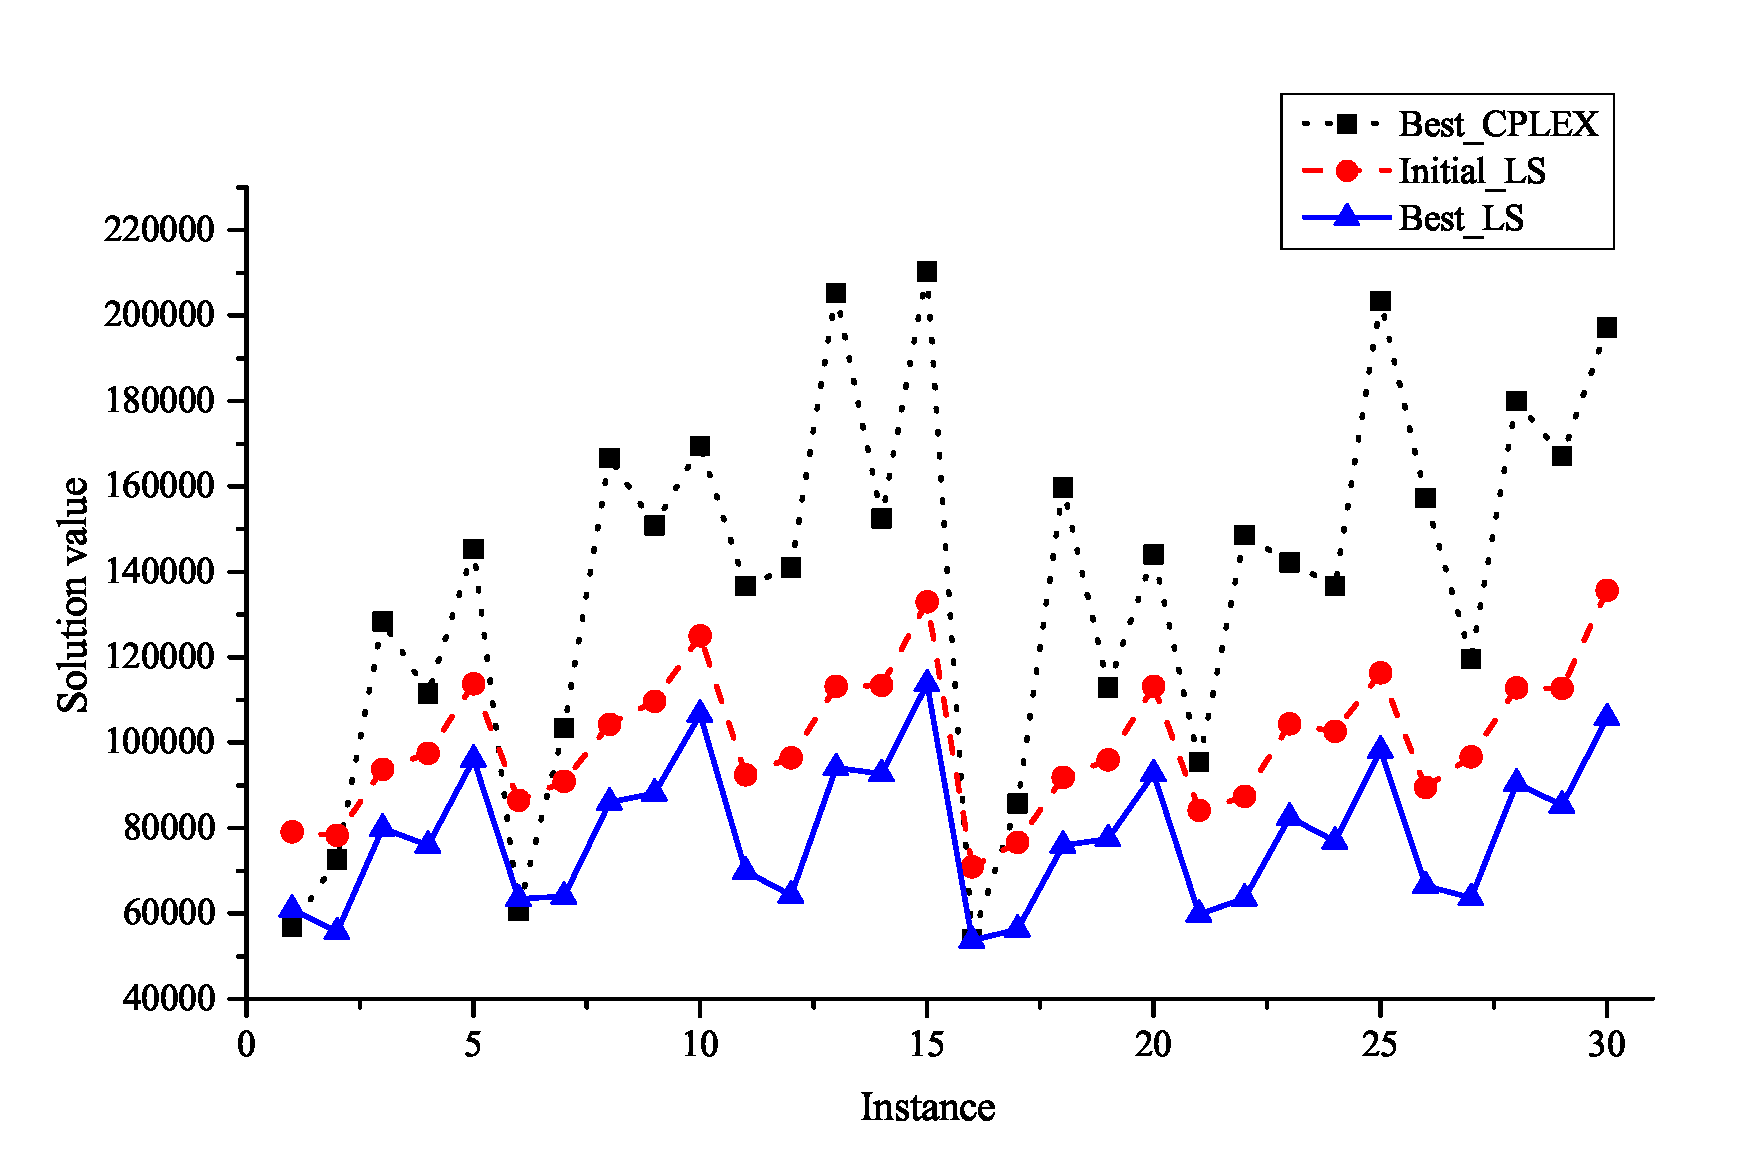
\includegraphics[width=0.9\linewidth]{F5.eps}
\caption{Comparative upper bounds of CPLEX and local search approach}
\label{threeUB}
\end{figure}

\subsubsection{Impact of heterogeneous fleet issue}
This section aims to examine the impact of heterogeneous fleet and demonstrate its necessity. In this respect, two small-scale test instances which can be solved optimally by CPLEX are randomly generated. Different numbers of fleet type provide transportation services over the two networks. We generate multiple combinations for each certain number of fleet type and take an average as the total cost. Main parameters of these networks and average total costs are shown in \autoref{heterogeneous}.

We employ \autoref{twoNetwork} to intuitively show the change of total costs as the number of fleet type increases. As \autoref{twoNetwork} illustrates, the diversification of fleet types reduces total cost over the same network. It is a reasonable result which accords with practical experience.

\begin{table}[H]
\setlength{\abovecaptionskip}{-3pt}
\setlength{\belowcaptionskip}{5pt}
\centering
  \footnotesize
  \caption{Parameters and total costs of two networks}
  \label{heterogeneous}

% Table generated by Excel2LaTeX from sheet 'Comparison'
\begin{tabular}{cccccccccc}
\hline
\multirow{2}[4]{*}{Network} & \multirow{2}[4]{*}{$|N|$} & \multirow{2}[4]{*}{$|K|$} & \multirow{2}[4]{*}{$|A|$} &       & \multicolumn{5}{c}{$|F|$} \bigstrut\\
\cline{6-10}      &       &       &       &       & 1     & 3     & 5     & 7     & 10 \bigstrut\\
\hline
1     & 8     & 15    & 50    &       & 4606.00  & 4074.13  & 3815.17  & 3745.50  & 3726.00  \bigstrut[t]\\
2     & 10    & 20    & 90    &       & 5569.20  & 4898.63  & 4625.83  & 4540.00  & 4527.00  \bigstrut[b]\\
\hline
\end{tabular}%

\end{table}%

\begin{figure}[H]
\setlength{\abovecaptionskip}{-5pt}
\setlength{\belowcaptionskip}{-5pt}
\centering
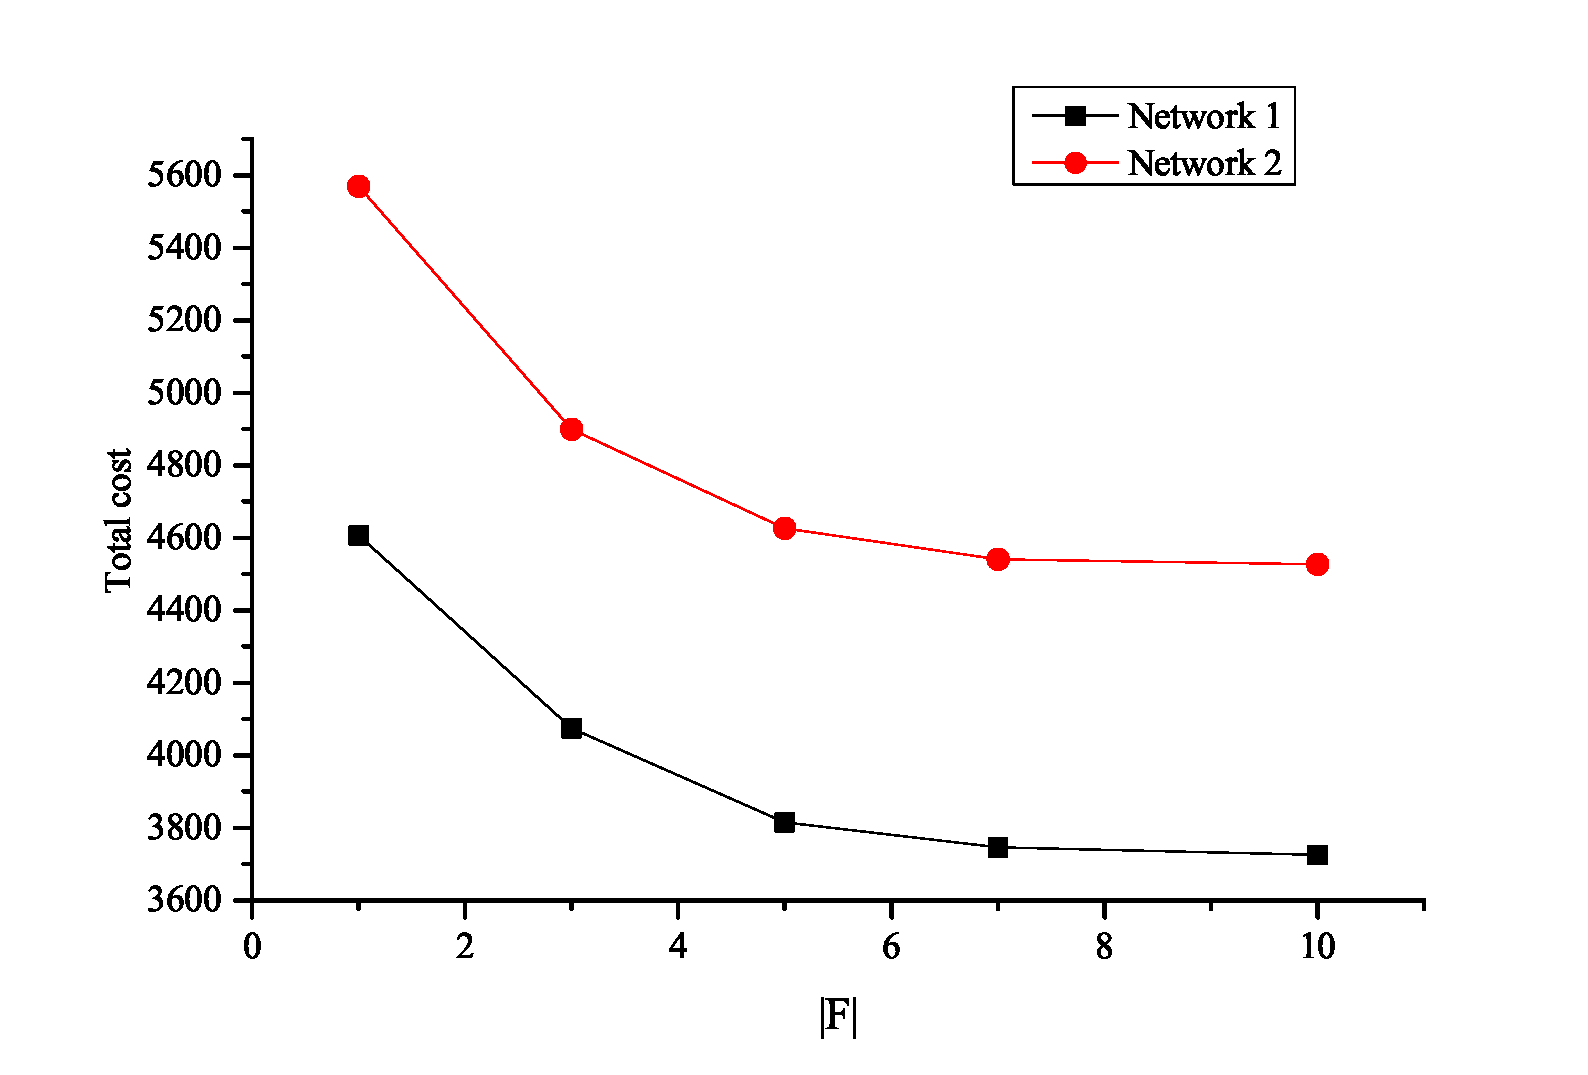
\includegraphics[width=0.9\linewidth]{F6.eps}
\caption{Change of total costs as $|F|$ increases}
\label{twoNetwork}
\end{figure}

\section{Conclusions}\label{conclusion}
We address heterogeneous fleet issue for service network design problem to accord with the real-life demand of transportation carriers and present two equivalent formulations based on arc and cycle-path respectively. Faced with increasingly huge logistics network, carriers are in urgent need of effective and efficient algorithms to help reduce total cost. Therefore, a hybrid algorithm combing exact and heuristic techniques is introduced to solve the proposed formulations. The method includes a column-and-cut generation procedure to efficiently achieve tight lower bounds and a local search algorithm to find high-quality solutions.

The computational study indicates the merit of the proposed column-and-cut generation procedure in strengthening the lower bounds and providing a good neighborhood for the local search approach to identify high-quality initial feasible solutions. The results also show the effectiveness of cycle-based neighborhood in searching for promising solutions. Both exact and heuristic techniques are proved to outperform the state-of-the-art MIP solver CPLEX. This performance appears more remarkable when comparing the computational efforts required by identifying lower bounds and upper bounds for the large-scale instances. We also perform computational experiments to illustrate the impact of heterogeneous fleet issue. The results show that the diversification of fleet types help reduce total cost for carriers.
\section*{Acknowledgments}

This work was supported by the National Natural Science Foundation of China
\bibliographystyle{ormsv080} % outcomment this and next line in Case 1
\bibliography{References} % if more than one, comma separated
\end{document}
